\documentclass[12pt]{article}
\usepackage{amsmath,amssymb}
\usepackage{physics}
\usepackage{geometry}
\geometry{margin=1in}
\usepackage{tikz}
\usetikzlibrary{arrows.meta,calc,angles,quotes}

\begin{document}

\begin{center}
\Large \textbf{Advanced Integrated Physics Problem Set — ULTRA HARD VERSION}\\
\large (Top 0.1\% JEE Advanced / IAT Elite Level)\\
\large Single Correct — 4 Options Each
\end{center}

\bigskip

%%%%%%%%%%%%%%%%%%%%%%%%%%%%%%%%%%%%%%%%%%%%%%%%%%%%%%%%%%%%

\textbf{Q1. Rotating Charged Bead with Gravitational and Magnetic Coupling [Diagram Required]}

A bead of mass $m$ and \textbf{positive} charge $q$ is constrained to move without friction on a rigid circular ring of radius $R$. The ring rotates with constant angular speed $\omega$ \textbf{counterclockwise as viewed from above} about a vertical diameter lying in the plane of the ring and passing through its center while a uniform magnetic field $ \vec B = B\hat z $ (directed upward) is present. Gravity acts vertically downward. The angular coordinate $\theta$ is measured from the lowest point of the ring.

Taking into account Coriolis effects, magnetic Lorentz force projection along the constraint, and equilibrium shift due to rotation, determine the frequency of small oscillations about the stable equilibrium position.

\begin{center}
\begin{tikzpicture}[scale=1]

% Vertical ring (in plane of page)
\draw (0,0) circle (2);

% Vertical diameter (axis of rotation)
\draw[dashed] (0,-2)--(0,2);
\node at (-0.4,2.4){$\omega$};

% Magnetic field upward
\draw[->,thick] (3,0)--(3,1.5);
\node at (3,1.8){$B\hat z$};

% Gravity downward
\draw[->] (-3,1.5)--(-3,0);
\node at (-3,1.8){$g$};

% Bead position
\fill (50:2) circle (2pt);
\node at (55:2.4){Bead};

% Radius line
\draw[dashed] (0,0)--(50:2);

% Theta measured from lowest point
\draw (0,-2) ++(0:0.5) arc (0:50:0.5);
\node at (25:1.2){$\theta$};

\end{tikzpicture}
\end{center}

\begin{enumerate}
\item[(A)] $\sqrt{\frac{g}{R}-\omega^2+\frac{qB\omega}{m}}$
\item[(B)] $\sqrt{\frac{g}{R}-\omega^2-\frac{qB\omega}{m}}$
\item[(C)] $\sqrt{\frac{g}{R}+\omega^2-\frac{qB\omega}{m}}$
\item[(D)] $\sqrt{\frac{g}{R}+\omega^2+\frac{qB\omega}{m}}$
\end{enumerate}

%%%%%%%%%%%%%%%%%%%%%%%%%%%%%%%%%%%%%%%%%%%%%%%%%%%%%%%%%%%%

\textbf{Q2. Central Potential with Inverse-Square Correction}

A particle of mass $m$ moves under a central potential  

\[
U(r)= -\frac{k}{r} + \frac{\alpha}{2r^2}
\]

where $k>0$ and $\alpha$ may be positive or negative. A circular orbit exists at radius $r_0$ corresponding to angular momentum conservation.  

Using effective potential curvature and stability criterion, determine the radial oscillation frequency for small perturbations about the circular orbit.

\begin{enumerate}
\item[(A)] $\sqrt{\frac{k}{mr_0^3}-\frac{3\alpha}{mr_0^4}}$
\item[(B)] $\sqrt{\frac{k}{mr_0^3}+\frac{3\alpha}{mr_0^4}}$
\item[(C)] $\sqrt{\frac{3k}{mr_0^3}-\frac{\alpha}{mr_0^4}}$
\item[(D)] $\sqrt{\frac{3k}{mr_0^3}+\frac{\alpha}{mr_0^4}}$
\end{enumerate}

%%%%%%%%%%%%%%%%%%%%%%%%%%%%%%%%%%%%%%%%%%%%%%%%%%%%%%%%%%%%

\textbf{Q3. Radial Oscillations in Rotating Groove with Elastic Constraint}

A particle of mass $m$ is constrained to move along a smooth radial groove cut in a horizontal disc rotating with constant angular speed $\omega$. The particle is connected to the center by a light spring of stiffness $k$ and natural length negligible compared to equilibrium position.  

Considering centrifugal equilibrium and restoring force linearization, determine the angular frequency of small radial oscillations about equilibrium.

\begin{enumerate}
\item[(A)] $\sqrt{\frac{k}{m}-\omega^2}$
\item[(B)] $\sqrt{\frac{k}{m}-2\omega^2}$
\item[(C)] $\sqrt{\frac{k}{m}+\omega^2}$
\item[(D)] $\sqrt{\frac{k}{m}-3\omega^2}$
\end{enumerate}

%%%%%%%%%%%%%%%%%%%%%%%%%%%%%%%%%%%%%%%%%%%%%%%%%%%%%%%%%%%%

\textbf{Q4. Sliding Conducting Rod with Electromagnetic Back Reaction [Diagram Required]}

A conducting rod of length $L$ and mass $m$ slides down parallel frictionless rails inclined at angle $\alpha$ with horizontal. The rails are connected through a resistor $R$, forming a closed circuit. A uniform magnetic field $B$ is directed perpendicular to the plane of rails.  

Accounting for motional emf, induced current, magnetic braking force, and steady state energy balance, determine the terminal velocity of the rod.

% Q4 Diagram
\begin{center}
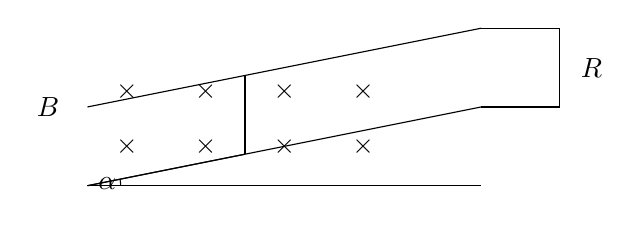
\begin{tikzpicture}[scale=1]

% Rails
\draw (0,0)--(5,1);
\draw (0,1)--(5,2);

% Rod
\draw[thick] (2,0.4)--(2,1.4);

% Resistor
\draw (5,1)--(6,1);
\draw (6,1)--(6,2);
\draw (6,2)--(5,2);
\node at (6.4,1.5){$R$};

% Correct angle alpha matching rail slope
\coordinate (A) at (0,0);
\coordinate (B) at (5,1);
\coordinate (H) at (5,0);

\draw (A) -- (H);
\draw (A) -- ($(A)!0.4!(B)$);

\pic [draw, angle radius=12pt, "$\alpha$"] {angle = H--A--B};
% B field crosses
\foreach \x in {0.5,1.5,2.5,3.5}
{
\foreach \y in {0.5,1.2}
{
\node at (\x,\y){$\times$};
}
}

\node at (-0.5,1){$B$};

\end{tikzpicture}
\end{center}

\begin{enumerate}
\item[(A)] $\frac{mgR\sin\alpha}{B^2L^2}$
\item[(B)] $\frac{mgR\sin\alpha}{2B^2L^2}$
\item[(C)] $\frac{2mgR\sin\alpha}{B^2L^2}$
\item[(D)] $\frac{mgR\sin\alpha}{\pi B^2L^2}$
\end{enumerate}

%%%%%%%%%%%%%%%%%%%%%%%%%%%%%%%%%%%%%%%%%%%%%%%%%%%%%%%%%%%%

\textbf{Q5. Two-Mass Spring System on Rotating Platform}

Two identical masses $m$ are connected by a light spring of stiffness $k$ and placed on a smooth horizontal turntable rotating with constant angular speed $\omega$. The midpoint of the spring coincides with the axis of rotation and remains fixed.  

By analyzing motion in rotating frame including centrifugal potential and symmetry constraints, determine the frequency of symmetric normal mode oscillation.

\begin{enumerate}
\item[(A)] $\sqrt{\frac{2k}{m}-\omega^2}$
\item[(B)] $\sqrt{\frac{2k}{m}-2\omega^2}$
\item[(C)] $\sqrt{\frac{k}{m}-\omega^2}$
\item[(D)] $\sqrt{\frac{k}{m}-2\omega^2}$
\end{enumerate}

%%%%%%%%%%%%%%%%%%%%%%%%%%%%%%%%%%%%%%%%%%%%%%%%%%%%%%%%%%%%

\textbf{Q6. Parallel Plate Capacitor with Movable Plate (Fixed Charge)}

A parallel plate capacitor with plate area $A$ and instantaneous separation $d$ carries a fixed charge $Q$. One plate of mass $m$ is attached to a spring of stiffness $k$ allowing motion along the normal direction while the other plate is fixed.  

Considering electrostatic energy dependence on separation and effective restoring force modification, determine the small oscillation frequency about equilibrium.

\begin{enumerate}
\item[(A)] $\sqrt{\frac{k}{m}+\frac{Q^2}{2\epsilon_0Am d^3}}$
\item[(B)] $\sqrt{\frac{k}{m}-\frac{Q^2}{2\epsilon_0Am d^3}}$
\item[(C)] $\sqrt{\frac{k}{m}+\frac{Q^2}{\epsilon_0Am d^3}}$
\item[(D)] $\sqrt{\frac{k}{m}-\frac{Q^2}{\epsilon_0Am d^3}}$
\end{enumerate}

%%%%%%%%%%%%%%%%%%%%%%%%%%%%%%%%%%%%%%%%%%%%%%%%%%%%%%%%%%%%

\textbf{Q7. Rolling Disc Inside Vertical Circular Track [Diagram Required]}

A uniform disc of radius $r$ rolls without slipping inside a fixed vertical circular hoop of radius $R$. The disc is given angular speed at the lowest point such that it moves along the inner surface.  

Using rolling constraint, energy conservation, and normal reaction condition at topmost point, determine the minimum angular speed \textbf{at the lowest point} required for the disc to just maintain contact at the highest point.
\begin{center}
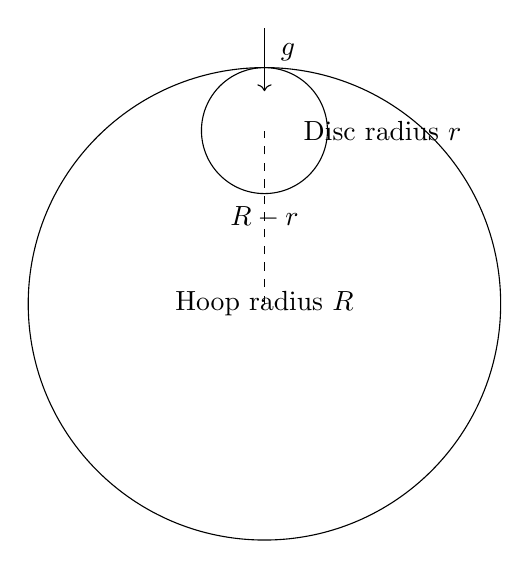
\begin{tikzpicture}[scale=1]

% Hoop center
\coordinate (O) at (0,0);

% Hoop
\draw (O) circle (3);

% Disc center at top (distance R-r = 3 - 0.8 = 2.2)
\coordinate (C) at (0,2.2);
\draw (C) circle (0.8);

% Centers connection
\draw[dashed] (O)--(C);

% Labels
\node at (0,0){Hoop radius $R$};
\node at (1.5,2.2){Disc radius $r$};
\node at ($(O)!0.5!(C)$) {$R-r$};

% Gravity
\draw[->] (0,3.5)--(0,2.7);
\node at (0.3,3.2){$g$};

\end{tikzpicture}
\end{center}

\begin{enumerate}
\item[(A)] $\omega^2>\dfrac{10g}{3(R-r)}$
\item[(B)] $\omega^2>\dfrac{11g}{3(R-r)}$
\item[(C)] $\omega^2>\dfrac{4g}{R-r}$
\item[(D)] $\omega^2>\dfrac{3g}{R-r}$
\end{enumerate}

%%%%%%%%%%%%%%%%%%%%%%%%%%%%%%%%%%%%%%%%%%%%%%%%%%%%%%%%%%%%

\textbf{Q8. Orbital Decay under Weak Tangential Drag}

A satellite of mass $m$ moves in a circular orbit of radius $r_0$ around a planet of mass $M$. A small tangential drag force proportional to gravitational force acts as  

\[
F = -\epsilon \frac{GMm}{r^2}, \quad \epsilon \ll 1.
\]

Using orbital energy loss per revolution and perturbative approximation, determine the fractional decrease in orbital radius after one complete revolution.

\begin{enumerate}
\item[(A)] $-4\pi\epsilon$
\item[(B)] $-2\pi\epsilon$
\item[(C)] $-\pi\epsilon$
\item[(D)] $-\dfrac{4\pi\epsilon}{3}$
\end{enumerate}

%%%%%%%%%%%%%%%%%%%%%%%%%%%%%%%%%%%%%%%%%%%%%%%%%%%%%%%%%%%%

\textbf{Q9. Combined Harmonic and Coulomb Central Force}

A particle moves under potential  

\[
U(r)=\frac12 kr^2 - \frac{\alpha}{r}.
\]

A stable circular orbit exists at radius $r_0$. Using effective potential curvature method and equilibrium condition, determine the radial oscillation frequency for small perturbations.

\begin{enumerate}
\item[(A)] $\sqrt{\frac{3k}{m}+\frac{\alpha}{mr_0^3}}$
\item[(B)] $\sqrt{\frac{k}{m}+\frac{3\alpha}{mr_0^3}}$
\item[(C)] $\sqrt{\frac{3k}{m}-\frac{\alpha}{mr_0^3}}$
\item[(D)] $\sqrt{\frac{k}{m}-\frac{3\alpha}{mr_0^3}}$
\end{enumerate}

%%%%%%%%%%%%%%%%%%%%%%%%%%%%%%%%%%%%%%%%%%%%%%%%%%%%%%%%%%%%

\textbf{Q10. Sliding Charged Block on Movable Wedge in Magnetic Field [Diagram Required]}

A wedge of mass $M$ rests on a frictionless horizontal surface. A block of mass $m$ and positive charge $q$ slides \textbf{down the incline} with instantaneous speed $v$ along its smooth surface of angle $\theta$ while a uniform magnetic field is directed into the page. The positive $x$-direction is taken toward the right.  

Considering constraint forces, induced horizontal motion of wedge, and Lorentz force components along constraint, determine instantaneous horizontal acceleration of the wedge.

\begin{center}
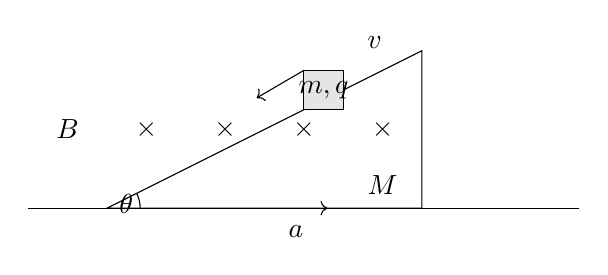
\begin{tikzpicture}[scale=1]

% Ground
\draw (-1,0)--(6,0);

% Wedge
\draw (0,0)--(4,0)--(4,2)--cycle;

% Block
\draw[fill=gray!20] (2.5,1.25) rectangle (3,1.75);
\node at (2.75,1.5){$m,q$};

% Angle theta
\coordinate (A) at (4,0);
\coordinate (B) at (0,0);
\coordinate (C) at (4,2);

\pic [draw, angle radius=12pt, "$\theta$"] {angle = A--B--C};

% Magnetic field crosses
\foreach \x in {0.5,1.5,2.5,3.5}
{
\node at (\x,1){$\times$};
}
\node at (-0.5,1){$B$};

% Wedge mass
\node at (3.5,0.3){$M$};

% Velocity arrow of block along incline
\draw[->] (2.5,1.75)--(1.9,1.4);
\node at (3.4,2.1){$v$};

% Horizontal acceleration of wedge
\draw[->] (2,0)--(2.8,0);
\node at (2.4,-0.3){$a$};

\end{tikzpicture}
\end{center}

\begin{enumerate}
\item[(A)] $\frac{mg\sin\theta\cos\theta}{M+m\sin^2\theta}$
\item[(B)] $\frac{mg\sin\theta\cos\theta}{M+m}$
\item[(C)] $\frac{mg\sin\theta\cos\theta-qBv\sin\theta}{M+m\sin^2\theta}$
\item[(D)] $\frac{mg\sin\theta\cos\theta+qBv\sin\theta}{M+m\sin^2\theta}$
\end{enumerate}

%%%%%%%%%%%%%%%%%%%%%%%%%%%%%%%%%%%%%%%%%%%%%%%%%%%%%%%%%%%%

\textbf{Q11. Axial Stability of Charge at Center of Charged Ring}

A particle of charge $q$ is placed at the center of a uniformly charged ring of total charge $Q$ and radius $R$. The particle is constrained to move along the axis perpendicular to the plane of the ring.  

Using Taylor expansion of electric field near center and restoring force approximation, determine the small oscillation frequency.

\begin{enumerate}
\item[(A)] $\sqrt{\frac{kQq}{mR^3}}$
\item[(B)] $\sqrt{\frac{2kQq}{mR^3}}$
\item[(C)] $\sqrt{\frac{kQq}{2mR^3}}$
\item[(D)] $\sqrt{\frac{3kQq}{mR^3}}$
\end{enumerate}

%%%%%%%%%%%%%%%%%%%%%%%%%%%%%%%%%%%%%%%%%%%%%%%%%%%%%%%%%%%%

\textbf{Q12. Falling Conducting Loop Entering a Finite Time-Varying Magnetic Field Region [Diagram Required]}

A square conducting loop of side $a$, mass $m$, and resistance $R$ falls vertically under gravity. The magnetic field exists only in the region $y>0$ and varies with time as  

\[
B(t)=B_0 t
\]

directed perpendicular to the plane of the loop (into the page).  

The loop is initially completely above the boundary and gradually enters the magnetic field region while falling.

Considering induced emf due to both motion and explicit time variation of the magnetic field, determine the terminal velocity reached after long time in the regime where $B_0 t$ becomes sufficiently large so that the velocity-dependent contribution to the induced emf dominates.
At terminal stage, only the horizontal segment of the loop lying inside the magnetic region contributes a net upward magnetic force opposing motion.

% Corrected Q12 Diagram
\begin{center}
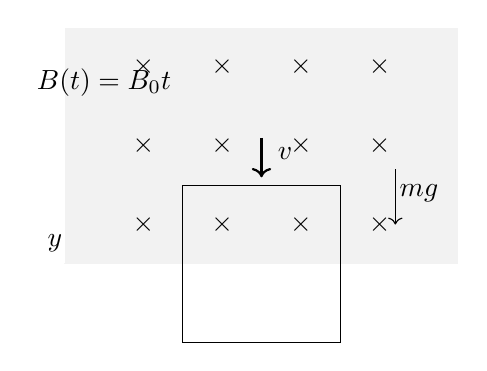
\begin{tikzpicture}[scale=1]

% Boundary line
\draw (-1,2)--(4,2);
\node at (-0.8,2.3){$y=0$};

% Field region shading
\fill[gray!10] (-1,2) rectangle (4,5);

% B field crosses (only above boundary)
\foreach \x in {0,1,2,3}
{
\foreach \y in {2.5,3.5,4.5}
{
\node at (\x,\y){$\times$};
}
}

\node at (-0.5,4.3){$B(t)=B_0 t$};

% Loop (partially inside region)
\draw (0.5,1) rectangle (2.5,3);

% Downward motion
\draw[->,thick] (1.5,3.6)--(1.5,3.1);
\node at (1.8,3.4){$v$};

% Gravity
\draw[->] (3.2,3.2)--(3.2,2.5);
\node at (3.5,2.9){$mg$};

\end{tikzpicture}
\end{center}

\begin{enumerate}
\item[(A)] $\dfrac{mgR}{B_0^2a^2}$
\item[(B)] $\dfrac{mgR}{2B_0^2a^2}$
\item[(C)] $\dfrac{2mgR}{B_0^2a^2}$
\item[(D)] $\dfrac{mgR}{4B_0^2a^2}$
\end{enumerate}

%%%%%%%%%%%%%%%%%%%%%%%%%%%%%%%%%%%%%%%%%%%%%%%%%%%%%%%%%%%%

\textbf{Q13. Coupled Electromechanical Oscillator with LC Circuit}

A capacitor of an LC circuit has one movable plate of mass $m$ attached to a spring of stiffness $k$. The battery is disconnected after charging, so total charge remains constant.  

Accounting for coupling between electrical and mechanical energy and linearizing about the static equilibrium separation of the plates, determine the lower normal mode frequency of the coupled system.

\begin{enumerate}
\item[(A)] $\sqrt{\frac{k}{m}}$
\item[(B)] $\sqrt{\frac{k}{m}-\frac{Q^2}{mC^2d^2}}$
\item[(C)] $\sqrt{\frac{k}{m}+\frac{Q^2}{mC^2d^2}}$
\item[(D)] $\sqrt{\frac{k}{m}-\frac{2Q^2}{mC^2d^2}}$
\end{enumerate}

%%%%%%%%%%%%%%%%%%%%%%%%%%%%%%%%%%%%%%%%%%%%%%%%%%%%%%%%%%%%

\textbf{Q14. Circular Motion in Rotating Frame with Gravitational Attraction}

A particle of mass $m$ moves radially in a frame rotating with angular speed $\omega$ about a fixed massive body of mass $M$. Both centrifugal and gravitational potentials act simultaneously.  

Using equilibrium condition in rotating frame and effective potential analysis, determine radius of stable circular orbit.

\begin{enumerate}
\item[(A)] $\left(\frac{GM}{\omega^2}\right)^{1/3}$
\item[(B)] $\left(\frac{2GM}{\omega^2}\right)^{1/3}$
\item[(C)] $\left(\frac{GM}{2\omega^2}\right)^{1/3}$
\item[(D)] $\left(\frac{3GM}{\omega^2}\right)^{1/3}$
\end{enumerate}

%%%%%%%%%%%%%%%%%%%%%%%%%%%%%%%%%%%%%%%%%%%%%%%%%%%%%%%%%%%%


\textbf{Q15. Circular Motion under Combined Gravitational and Magnetic Fields}

A particle of mass $m$ and positive charge $q$ moves in a circular orbit of radius $r$ around a massive body of mass $M$. The orbital motion is counterclockwise as viewed from above. A uniform magnetic field is directed upward (along $+\hat z$), perpendicular to the orbital plane.

Considering the direction of Lorentz force relative to gravitational attraction and centripetal requirement, determine the equation governing orbital speed.

\begin{enumerate}
\item[(A)] $\frac{mv^2}{r}=\frac{GMm}{r^2}+qvB$
\item[(B)] $\frac{mv^2}{r}=\frac{GMm}{r^2}-qvB$
\item[(C)] $\frac{mv^2}{r}=\frac{GMm}{r^2}+\frac{qvB}{2}$
\item[(D)] $\frac{mv^2}{r}=\frac{GMm}{r^2}-\frac{qvB}{2}$
\end{enumerate}

%%%%%%%%%%%%%%%%%%%%%%%%%%%%%%%%%%%%%%%%%%%%%%%%%%%%%%%%%%%%

\end{document}